\chapter{Reference model\label{sec:reference_model}}
\par{
    As a reference to compare the models trained on weakly-supervised data with, the model performance of a model trained on the same fully supervised data is taken as a reference.
    In this chapter, the results of these fully supervised reference experiments are discussed.
    The metric based on which the experiment results are compared is the weighted dice score, see equation \ref{eq:weighted_dice} on page \pageref{eq:weighted_dice}.
}

\section{Experiment results}
\par{
    The fully supervised experiments serve two goals.
    First is to calculate a reference model performance with which to compare the weakly supervised model results.
    The second is to support hyperparameter choices for the point supervised experiments.
    It is assumed that a network architecture that yields a good fully supervised model is also a suitable choice to build a weakly supervised model.
    The possible influence of the context slices\footnote{The context slice idea is discussed in detail in chapter \ref{section:twoDplus} on page \pageref{section:twoDplus}.} is also evaluated with these experiments.
}
\par{
    In figure \ref{fig:referenceExperiments}, the results of the reference experiments are shown.
    These results show the network based on VGG16 yields better results than the alternatives based on RESNET50 and U-Net.
    Despite what was hoped for, the context slices do not seem to increase the model performance.
    Remarkably, there is little difference between the models trained with a weighted cross-entropy loss and the non-weighted cross-entropy loss.
}
\begin{SCfigure}[][htb]
    \centering
    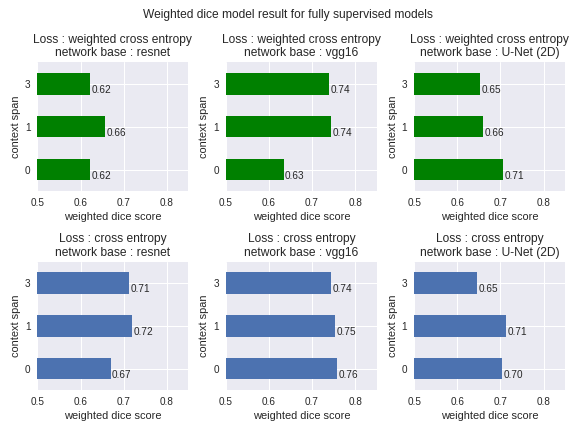
\includegraphics[width=.95\textwidth]{images/FullySupervised.png}
    \caption{Results of the fully supervised experiments.
    The indicated model performance metrics are calculated on the test set.
    \label{fig:referenceExperiments}}
\end{SCfigure}

\todo[inline]{
    Assure the models are fully converged. 
    Express this uncertainty on the results --> mention the need to decide under time pressure.
}

\section{Conclusion}
Based on the results shown in figure \ref{fig:referenceExperiments}, it was decided to perform the weakly supervised experiments with the model based on VGG16 FCN8 with 1 context slice.